% !TEX root = thesis.tex

\section{Optimizing Higher-Order Functions in MATLAB}
\label{se:CS-matlab}

In this section we show how \osrkit\ can be used in a production VM to implement aggressive optimizations for dynamic languages; in particular, we focus on MATLAB, a popular dynamic language for scientific and numerical programming.

Introduced in the late 1970s mainly as a scripting language for performing computations through efficient libraries, MATLAB has evolved over the years into a more complex programming language with support for high-level features such as functions, packages and object orientation. A popular feature of the language is the \feval\ construct, a built-in higher-order function that applies the function passed as first parameter to the remaining arguments (e.g., {\tt feval(g,x,y)} computes {\tt g(x,y)}). This feature is heavily used in many classes of numerical computations, such as iterative methods for approximate solutions of an ordinary differential equation (ODE) and simulated annealing heuristics to locate a good approximation to the global optimum of a function in a large search space.

A previous study by Lameed and Hendren~\cite{Lameed2013b} shows that the overhead of an \feval\ call is significantly higher than a direct call, especially in JIT-based execution environments such as McVM~\cite{Chevalier2010} and the proprietary MATLAB JIT accelerator by Mathworks. In fact, the presence of an \feval\ instruction can disrupt the results of intra- and inter-procedural level for type and array shape inference analyses, which are key factors for efficient code generation. Furthermore, since \feval\ invocations typically require a fallback to an interpreter, parameters passed to an \feval\ are typically boxed to make them more generic.

Our case study presents a novel technique for optimizing \feval\ in the McVM virtual machine, a complex research project developed at McGill University. McVM is publicly available~\cite{mcvm} and includes: a front-end for lowering MATLAB programs to an intermediate representation called IIR that captures the high-level features of the language; an interpreter for running MATLAB functions and scripts in IIR format; a manager component to perform analyses on IIR; a JIT compiler based on LLVM for generating native code for a function, lowering McVM IIR to LLVM IR; a set of helper components to perform fast vector and matrix operations using optimized libraries such as ATLAS, BLAS and LAPACK. %The architecture of McVM is illustrated in Figure [...]

McVM implements a function versioning mechanism based on type specialization, which is the main driver for generating efficient code~\cite{Chevalier2010}: for each IIR representation of a function, different IR versions are generated according to the types of the arguments at each call site. The number of generated versions per function is on average small (i.e., less than two), as in most cases functions are always called with the same argument types.

\subsection{Current Approaches}
\label{ss:CS-prev-eval-sol}

Lameed and Hendren~\cite{Lameed2013b} proposed two dynamic techniques for optimizing \feval\ instructions in McVM: {\em JIT-based} and {\em OSR-based} specialization. Both attempt to optimize a function $f$ that contains instructions of the form \feval$(g,...)$, leveraging information about $g$ and the type of its arguments observed at run time. The optimization produces a specialized version $f'$ where \feval$(g,x,y,z,...)$ instructions are replaced with direct calls of the form $g(x,y,z,...)$. 

The two approaches differ in the points where code specialization is performed. In JIT-based specialization, $f'$ is generated when $f$ is called. In contrast, the OSR-based method interrupts $f$ as it executes, generates a specialized version $f'$, and resumes from it.  

Another technical difference, which has substantial performance implications, is the representation level at which optimization occurs in the two approaches. When a function $f$ is first compiled from MATLAB to IIR, and then from IIR to IR, the functions it calls via \feval\ are unknown and the type inference engine is unable to infer the types of their returned values. Hence, these values must be kept boxed in heap-allocated objects and handled with slow generic instructions in the IR representation of $f$ (suitable for handling different types).

The JIT method works on the IIR representation of $f$ and can resort to the full power of type analysis to infer the types of the returned values of $g$, turning the slow generic instructions of $f$ into fast type-specialized instructions in $f'$. When $g$ is one of the parameters of $f$, each call to $f$ can be redirected to a dispatcher that evaluates at run-time the value of the argument to use for the \feval\ and executes either a previously compiled cached code or generates and JIT-compiles a version of the function optimized for the current value.

On the other hand, OSR-based specialization operates on the IR representation of $f$, which prevents the optimizer from exploiting type inference. As a consequence, for $f'$ to be sound, the direct call to $g$ must be guarded by a condition that checks whether the type of its parameters remain the same as observed at the time when $f$ was interrupted. If the guard fails, or the \feval\ target $g$ changes, the code falls back to executing the original \feval\ instruction.

JIT-based specialization is substantially faster than OSR-based specialization due to the benefits of type inference, but is less general as it only works if the \feval\ argument $g$ is one of the parameters of $f$. JIT-based specialization thus cannot be applied to scenarios where, e.g.:
\begin{itemize}[itemsep=0pt,parsep=3pt,partopsep=0pt]
\item $f$ is an {\tt inline} or an anonymous function defined in $g$;
\item $f$ is the return value from a previous call in $g$ to another function;
\item $f$ is retrieved from a data structure~\cite{Lameed2013b};
\item $f$ is a constant string containing the name of a user-defined function (a rather common misuse of \feval\ among MATLAB users~\cite{Radpour2013}).
\end{itemize}

\subsection{A New Approach}
\label{ss:CS-new-eval-sol}

In this section, we present a new approach that combines the flexibility of OSR-based specialization with the efficiency of the JIT-based method, answering an open question raised by Lameed and Hendren~\cite{Lameed2013b}.

The key idea is to lift the $f$-to-$f'$ optimization performed by the OSR-based specialization from IR to IIR level. This makes it possible to perform type inference in $f'$, generating much more efficient code. The main technical challenge of this idea is that the program's state in $f$ at the OSR point may be incompatible with the state of $f'$ from which execution continues. Indeed, some variables may be boxed in $f$ and unboxed in $f'$. Hence, compensation code is needed to adjust the state by performing live variable unboxing during the OSR.

\subsubsection*{Implementation}

We implemented our approach in McVM\footnote{As a by-product of our project, we ported the MATLAB McVM virtual machine from the LLVM legacy JIT to the new MCJIT toolkit. Our code is available at \url{https://github.com/dcdelia/mcvm}.}, extending it with four main components:

\begin{enumerate}[itemsep=0pt,parsep=3pt]
\item An analysis pass to identify optimization opportunities for \feval\ instructions in the IIR of a function.
\item An extension for the IIR compiler to track the {\em variable map} between IIR and IR objects at \feval\ sites.
\item An OSR inserter based on \osrkit\ to inject open OSR points in the IR for IIR locations annotated during the analysis pass.
\item An \feval\ optimizer triggered at OSR points, which uses:
  \begin{enumerate}[itemsep=0pt,partopsep=0pt]
  \item a profile-driven IIR generator to replace \feval\ calls with direct calls;
  \item a helper component to lower the optimized IIR function to IR and construct a state mapping;
  \item a code caching mechanism to handle the compilation of the continuation functions.
  \end{enumerate}
\end{enumerate}

\noindent We remark that our implementation heavily depends on \osrkit's ability to handle compensation code. 

\paragraph*{Analysis Pass.} The analysis pass, which is fully integrated in McVM's analysis manager, groups \feval\ instructions whose first argument is reached by the same definition, and for each group marks for instrumentation only those instructions that are not dominated by others, so that the function can be optimized as early as possible at run time.
It also determines whether the value of the argument can change across two executions of the same \feval, and a run-time guard must thus be inserted during the optimization phase.

\paragraph*{IIR Compiler Extension.} The extension operates when the IIR compiler processes an annotated \feval\ instruction. It builds a {\em variable map} between IIR and IR objects, and keeps track of the {\tt llvm::BasicBlock*} $b$ created for the \feval\ in the IR code and of the {\tt llvm::Value*} object $g$ used as its first argument. 

\paragraph*{OSR Inserter.} The OSR inserter uses the $b$ and $g$ objects collected by the IIR compiler extension respectively as basic block and {\tt val} argument for the open-OSR stub (\mysection\ref{ss:osrkit-implementation}) that invokes the \feval\ optimizer.

\newcommand{\fBase}{$f$}
\newcommand{\fOpt}{$f_{opt}$}
\newcommand{\fIIR}{$f^{IIR}$}
\newcommand{\fIR}{$f^{IR}$}
\newcommand{\fOptIIR}{$f^{IIR}_{opt}$}
\newcommand{\fOptIR}{$f^{IR}_{opt}$}
\newcommand{\gTarget}{$g$}

\paragraph*{Optimizer.} The core of our optimization pipeline is the optimizer module, which is called as {\tt gen} function in the open OSR stub created by the OSR inserter. It receives the IR version \fIR\ of function \fbase, the basic block of \fIR\ where the OSR was fired, and the native code address of the \feval\ target function \gTarget. As a first step, the optimizer looks up the IR code of \gTarget\ by its address and checks whether a previously compiled version of \fBase\ specialized with \gTarget\ was previously cached. If not, a new function \fOptIIR\ is generated by cloning the IIR representation \fIIR\ of \fBase\ and by replacing all \feval\ calls to \gTarget\ in \fOptIIR\ with direct calls.

As a next step, the optimizer asks the IIR compiler to lower \fOptIIR\ to \fOptIR. During the process, the compiler stores the variable map between IIR and IR objects at the direct call replacing the \feval\ instruction that triggered the OSR.

Using this map and the one stored during the lowering of \fIIR, the optimizer constructs a state mapping between \fIR\ and \fOptIR. In particular, for each value in \fOptIR\ live at the continuation block we determine whether we can assign to it a live value passed at the OSR point, or a compensation code is required to set its value.

Notice that since the type inference engine yields more accurate results for \fOptIIR\ compared to \fIIR, the IIR compiler can in turn generate efficient specialized IR code for representing and manipulating IIR variables, and compensation code is typically required to unbox or downcast some of the live values passed at the OSR point, or to materialize as an IR object an IIR variable previously accessed through \mytt{get}/{\mytt{set} methods from McVM's environment.

Once a state mapping has been constructed, the optimizer asks \osrkit\ to generate the continuation function for the OSR transition and then executes it, also storing the address of the compiled function in the internal code cache.

\ifdefined\noauthorea
\begin{figure}[!ht]
\begin{center}
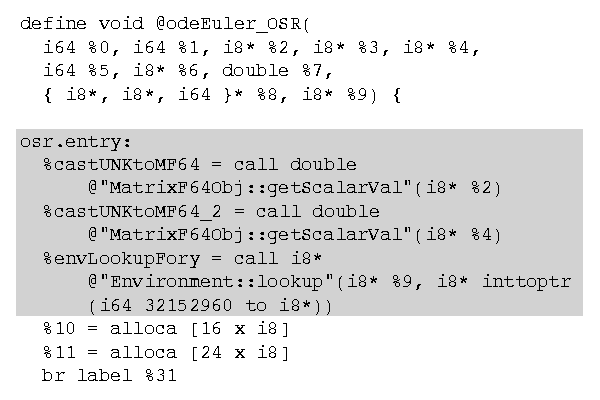
\includegraphics[width=0.7\columnwidth]{figures/CS-comp-code/CS-comp-code.eps}
\caption{\protect\label{fig:CS-comp-code} Compensation code for {\tt odeEuler} benchmark. McVM-specific instructions are highlighted in grey.%\label{fig:comp-code} Compensation code generated for {\tt odeEuler}. McVM instructions for unboxing variables to {\tt double} and fetching object {\tt y} from the environment are in grey. Two arrays of bytes are then allocated on the stack.
}
\end{center}
\end{figure}
\fi

\noindent An example of compensation code is reported in \myfigure\ref{fig:CS-comp-code}. In order to correctly resume the execution at the first instruction in basic block {\tt \%31}, the entrypoint of {\tt odeEuler}'s continuation function executes a sequence of instructions that: 1) convert to {\tt double} two live variables -- i.e., function arguments {\tt \%2} and {\tt \%4} -- that are represented as boxed values in the unoptimized function, 2) look up in McVM's environment at {\tt \%9} the pointer to the object instantiated for the symbol description stored at address {\tt 0x32152960}, and 3) allocate on the stack two buffers of 16 and 24 bytes, respectively.

\subsection{Performance Analysis}
We now analyze the impact of our optimization technique for \feval\ on the running time of a few numeric benchmarks, namely {\tt odeEuler}, {\tt odeMidpt}, {\tt odeRK4}, and {\tt sim\_anl}. The first three benchmarks~\cite{Recktenwald2000} solve an ordinary differential equation for heat treating simulation using the Euler, midpoint, and Range-Kutta method, respectively; the last benchmark minimizes the six-hump camelback function with the method of simulated annealing~\cite{simanl}.

We report the speedups enabled by our technique in \mytable\ref{tab:CS-feval}, using the running times for McVM's \feval\ default dispatcher as baseline. As the dispatcher typically JIT-compiles the invoked function, we also analyzed running times when the dispatcher calls a previously compiled function. In the last column, we show speedups from a modified version of the benchmarks in which each \feval\ call is replaced by hand with a direct call to the function in use for the specific benchmark.

Unfortunately, we are unable to compute direct performance metrics for the solution by Lameed and Hendren as its source code has not been released. Figures in their paper~\cite{Lameed2013b} show that for the very same MATLAB programs the speedup of the OSR-based approach is on average within $30.1\%$ of the speedup of hand-coded optimization (ranging from $9.2\%$ to $73.9\%$); for the JIT-based approach, the average grows to $84.7\%$ (ranging from $75.7\%$ to $96.5\%$).

\begin{table}[ht!]
\begin{center}
\vspace{4mm}
\begin{small}
% dirty hack for text wrapping
\begin{tabular}{ |c|c|c|c|c| }
\cline{2-5}
\multicolumn{1}{c|}{} & Base & Optimized & Optimized & Direct \\ 
\cline{1-1}
Benchmark & (cached) & (JIT) & (cached) & (by hand) \\
\hline
\hline
odeEuler & 1.046 & 2.796 & 2.800 & 2.828 \\ 
\hline
odeMidpt & 1.014 & 2.645 & 2.660 & 2.685 \\ 
\hline
odeRK4 & 1.005 & 2.490 & 2.582 & 2.647 \\ 
\hline
sim\_anl & 1.009 & 1.564 & 1.606 & 1.612 \\ 
\hline
\end{tabular}
\end{small}
\end{center}
\caption{\label{tab:CS-feval} Q4: Speedup comparison for \feval\ optimization.} 
\end{table}

\noindent Our optimization technique yields speedups that are very close to the upper bound given from by-hand optimization; in the worst case ({\tt odeRK4} benchmark), we observe a $94.1\%$ when the optimized code is generated on the fly, which becomes $97.5\%$ when a cached version is available. Compared to their OSR-based approach, the compensation entry block is a key driver of improved performance, as the benefits from a better type-specialized whole function body outweigh those from performing a direct call using boxed arguments and return values in place of the original \feval.

\noindent For the \mytt{sim\_anl} benchmark, \osrkit's support for OSR point insertion at arbitrary locations allowed our optimization pipeline to instrument an \feval\ instruction that occurs before the main loop and pollutes type inference information for the rest of the code: in fact, the OSR-based solution by Lameed and Hendren yielded a very limited performance improvement for this benchmark.

\subsection{Discussion}
The ideas presented in this case study advance the state of the art of \feval\ optimization in MATLAB runtimes.
%combine the flexibility of OSR-based specialization with the efficiency of the JIT-based method. 
Similarly to OSR-based specialization, we do not place restrictions on the functions that can be optimized. On the other hand, we work at IIR (rather than IR) level as in JIT-based specialization, which allows us to perform type inference on the code with direct calls. Working at IIR level eliminates the two main sources of inefficiency of OSR-based specialization:
\begin{enumerate}[partopsep=0pt,itemsep=0pt,parsep=3pt]
 \item we can replace generic instructions with specialized instructions, and
 \item the types of $g$'s arguments do not need to be cached or guarded as they are statically inferred.
\end{enumerate}

\noindent These observations are confirmed in practice by experiments on a number of typical benchmarks from the MATLAB community.